\fancychapter{User-centred Studies}
\label{chapter:user-studies}

The chosen \emph{Sueca} scenario gives this work an opportunity to study \ac{hri} with a senior audience in an entertainment activity.
However, developing a robot for aged people brings some delicate questions.
The potential users sometimes have few, or nonexistent, experience with technology, which makes it difficult for them to understand how robots work and what they can actually do.
As a result, understanding their needs, expectations, and fears is another concern \cite{Oliveira}.


The current chapter explains the methodology, procedures and current results of a developed user-centred study in a care home.
It involved two different activities, a focus group and a pilot card game study, as a result of two distinct motivations: to understand the elderly' concerns about robots, and to analyse both the game flow and the interactions between players during a \emph{Sueca} session of games.
%This aimed to collect specific social, verbal and nonverbal behaviours, and also some cognitive and strategic guidelines in the domain of \emph{Sueca}.
%Additionally, another goal of these user studies is to understand their needs, expectations, and fears \cite{Oliveira}. As a result, the following pilot study was developed in a care home in order to answer all these questions.


\section{Focus Group}

A focus group is a good approach for a first meeting due to the informal and conversational way of interacting with participants.
The goal of this activity was to introduce to the elderly the robots' theme, and to understand their opinions and expectations.
To accomplish this purpose, used techniques were a Brainstorming and a Storytelling.

\subsection{Methodology}
The elderly participants were divided into groups of 5.
There were 2 researchers per group commanding and guiding all the process.
The list of materials used, per group:

\begin{itemize}
\item An illustrative video of existing robots;
\item 6 photographs of different robots, including 3 of service type and 3 of companion type (Paro, EMYS, Pleo, Pearl, PR2, and Care-O-Bot);
\item Two white boards and three pens (black, red and green);
\item Three hypothetical stories of robots;
\item An audio recorder;
\item Four lavalier microphones;
\item A video camera.
\end{itemize}

The last three items will only be used for a further analysis of this focus group.
The video tries to answer the questions: what is a robot, what can robots do, how do they work, do they fail and how do science fiction movies present robots to us.
In order not to bias their thoughts, we tried to gather positive and negative aspects of existing robots.
The three hypothetical stories aim to bring ethical discussions to the focus group \cite{Kahn2006,Should2010}.
For instance, an elderly that owns a robot in his home tells him a secret.
If that robot is questioned about the secret, should it or should it not tell other people the truth?

\subsection{Procedures}
All the materials enumerated in the previous list were arranged as in Figure~\ref{fig:focus-group}.
Firstly, each person in the room briefly introduces himself in order to make everyone feeling more comfortable.
Secondly, the video is shown.
Then, everyone starts discussing about robots' purposes and they are registered in one of the white boards with the black coloured pen.
People also express a positive or negative impression of each robot's purpose and their opinions decide the colour of the surrounding line (Appendix).
For instance, the sentence ``Call an ambulance'' written on the board is surrounded by a green line if they think it is a good purpose for a robot.
After finishing this task, one of the group leaders writes all the sentences previously collected in the second board but without the surrounding green or red lines.
The other group leader starts reading the hypothetical stories and opens a new discussion about what the robots of each story should do.
He also presents the photographs and tries to understand which robot is more suitable for each purpose in their opinion.
When bringing the new board to the room, the idea is to understand if their positive and negative opinions about each purpose have changed.


\subsection{Results}

Three focus group sessions were performed and analysed, with 16 participants from a day-home care institution in Lisbon (12 females, 4 males; M age = 78.69 $\pm$ 12.20).
Most subjects lived alone in their home (81.3\%), or with their friends (12.5\%), and relatives (6.3\%).

The analyses focused on the mentioned activities in which independent-living older adults require a robot.
Out of 75 mentioned activities, 65 were non-repeated activities that were further classified according to their primary goal and context.
The used classification was: Basic Activities of Daily Living (BADL), Instrumental Activities of Daily Living (IADL), Enhanced Activities of Daily Living (EADL) and Social Activities (SA).
Consequently, the distribution of activities went as follows: 24 IADL, 17 BADL, 12 EADL and 12 SA.
These results evidenced how independent-living older adults expect robots might help to improve their quality of life, and also which type of activities they require the most.

Moreover, the analysis on the robot types demonstrated their preferences on service robots for each activity type. The main reason for this choice is their physicality, which is perceived as less limiting when compared to other robot types.

\begin{figure}
        \centering
        \begin{subfigure}[h]{0.49\textwidth}
                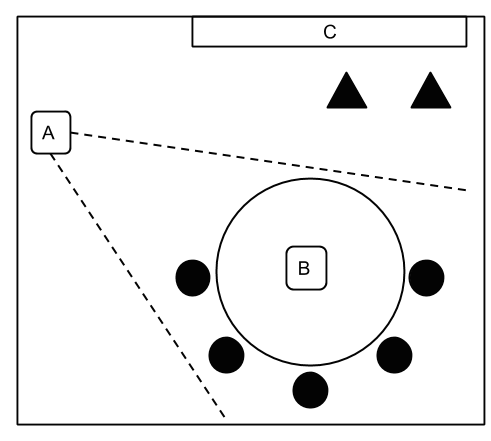
\includegraphics[width=\textwidth]{./img/5/focusGroup}
                \caption{Focus Group}
                \label{fig:focus-group}
        \end{subfigure}
        \begin{subfigure}[h]{0.49\textwidth}
                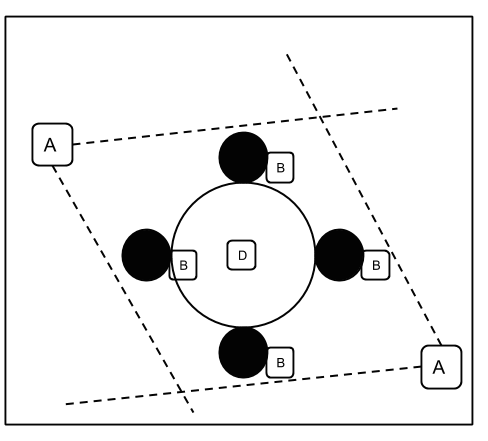
\includegraphics[width=\textwidth]{./img/5/cardGame}
                \caption{Card game}
                \label{fig:card-game}
        \end{subfigure}
        \caption[Setting of the user study activities.]{Setting of the user study activities. \textbf{A} - Video recorder \textbf{B} - Audio recorder / Microphone \textbf{C} - White board \textbf{D} - cards \ding{108} - Aged person \ding{115} - Group leader}\label{fig:user-studies}
\end{figure}





\section{Card Games}
The further reproduction of human behaviours, in the \emph{Sueca} domain, will be required for the social robotic agent.
Consequently, this user-centred study plays a crucial role in the following stages of this work.
Besides collecting examples of verbal and non-verbal interactions from human players, the analysis of these card games aimed to capture the precise game situations that trigger those behaviours.



\subsection{Methodology}
Considering each \emph{Sueca} card game includes four players, the required materials were: a card deck, a table and chairs for the four players, two video cameras and an audio recorder with four microphones.

\subsection{Procedures}
All the previously enumerated material was arranged as in the Figure~\ref{fig:card-game}.
Each video camera was positioned to capture the hands of two adjacent players.
Players were recorded during a tournament of several games.
They were told to play as long as they wanted with a maximum duration of one hour.

\subsection{Results}
The session took only 40 minutes, since the 4 players were feeling weary.
Ten games, with an average duration of 3,75' each, were recorded for a further analysis.
From the average duration, 1' belongs to the initial setting of shuffling, distributing, and rearranging the cards in each hand.

\begin{figure}[h]
  \centering
    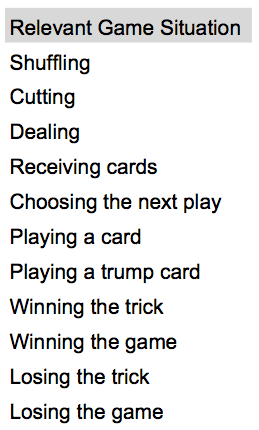
\includegraphics[width=0.2\textwidth]{./img/5/gameSituations}
  \caption{Relevant game situations extracted from the user-centred studies}
\label{fig:gameSituations}
\end{figure}

Figure~\ref{fig:gameSituations} lists all the captured game situations that trigger verbal and non-verbal behaviours.
Additionally, a player interacts when executing himself each action of the list or, also, when other player does it.
%As expected, players did not frequently talk during the game.
%\emph{Sueca} is indeed traditionally called as silent game.
%After a game, paired players frequently discuss extremely good or bad moves from each other.
%However, the analysis was focused mostly on interactions during the game.


\begin{table}[h]
\caption{Examples of expressions collected during the card game activity and its respective classification.}
\resizebox{\textwidth}{!}{%
\begin{tabular}{|l|m{0.3\textwidth}|m{0.3\textwidth}|}
\hline
\textbf{Expression} & \textbf{Game Stage} & \textbf{Intention} \\ \hline
\textit{Joga }{[}player-name{]}\textit{!} & Before a play & Speed up a play. \\ \hline
\textit{Anda }{[}player-name{]}\textit{!} & Before a play & Speed up a play. \\ \hline
\textit{Podes jogar, }{[}player-name{]}\textit{!} & Before a play & Speed up a play. \\ \hline
\textit{Quase que livr\'amos.} & After collecting the first points & Hopeful or ironic comment. \\ \hline
\textit{E eu puxo trunfo.} & Initialising a turn with a trump card & State an action. \\ \hline
\textit{Outro trunfo!} & Play a trump card after an already played trump card & State an action. \\ \hline
\textit{Outro(a) }{[}suit{]}\textit{!} & Play a {[}suit{]} card after an already played {[}suit{]} card & State an action. \\ \hline
\textit{O trunfo \'e }{[}suit{]}\textit{.} & Anytime & Give game information. Answer a question. \\ \hline
\end{tabular}
}
\label{tab:interactions}
\end{table}


Table~\ref{tab:interactions} illustrates the some of the collected expressions, their corresponding game situations and their intentions.
Considering players said specific domain words, expressions were not translated in order not to lose their meaning and regarding the future usage of these sentences in a Portuguese environment.

Furthermore, there were other relevant considerations from these games analysis.
After a game, paired players frequently discuss extremely good or bad moves from each other.
Also, their main gazing points were the table zone with the card being played and their hands.


\cleardoublepage


